%%%%%%%%%%%%%%%%%%%%%%%%%%%%%%%%%%%%%%%%%%%%%%%%%%%%%%%%%%%%%%%%%%%%%%%%%%%%%%%%%%%%%%%%%%%%%%%%%%%%
% ==================================================================================================
% --------------------------------------------------------------------------------------------------
\chapter{Maths}
This section presents various mathematical results which are not crucial to the thesis.
%%%%%%%%%%%%%%%%%%%%%%%%%%%%%%%%%%%%%%%%%%%%%%%%%%%%%%%%%%%%%%%%%%%%%%%%%%%%%%%%%%%%%%%%%%%%%%%%%%%%
\section{FLAIR MRI Intensity Modelling}\label{s:simflair}
While MR imaging is both complex and mutable, simulation of the expected signal intensities is possible using the relaxometry data in Table \ref{tab:t1t2tissues} and sequence signal equations -- e.g. (\ref{eq:MRI-SE}) and (\ref{eq:MRI-IR}). In the clinic, this simulation helps select appropriate acquisition parameters $TE/TR/TI$ for the desired contrast; however, these contrast characteristics can also be later considered as covariates in performance analysis of segmentation tools. To this end, the acquisition parameters of the FLAIR image database (Table \ref{tab:database}) were used with the data from Table \ref{tab:t1t2tissues} and Equation (\ref{eq:MRI-IR}) to calculate the expected tissue contrasts for these data. The contrast between two graylevels was defined as
\begin{equation}
2\left|\frac{y_1 - y_2}{y_1 + y_2}\right|.
\end{equation}
These results are summarized in Table \ref{tab:simflair}, and an example image is generated for each parameter set using the tissue maps from the BrainWeb database \cite{Collins1998}%
\footnote{\hreftt{http://brainweb.bic.mni.mcgill.ca/}}%
, as shown in Figure \ref{fig:simflair}.
\begin{table}[h]
  \centering
  \caption{Simulated FLAIR tissue contrasts using scan parameters from the experimental database.}
  \label{tab:simflair}
  \begin{tabular}{rcccccc}
  	\hline
  	Scanner      & \gm/\wm & \gm/\csf & \gm/\wmh & \wm/\csf & \wm/\wmh & \csf/\wmh \\ \hline
  	WMH 2017 (1) & 0.19    & 1.28     & 0.32     & 1.16     & 0.50     & 1.45      \\
  	WMH 2017 (2) & 0.10    & 1.83     & 0.14     & 1.81     & 0.25     & 1.85      \\
  	WMH 2017 (3) & 0.13    & 1.95     & 0.27     & 1.94     & 0.39     & 1.96      \\
  	MS  2016 (1) & 0.28    & 2.00     & 0.88     & 2.00     & 1.09     & 2.00      \\
  	MS  2016 (2) & 0.25    & 2.00     & 0.82     & 2.00     & 1.01     & 2.00      \\
  	MS  2016 (3) & 0.32    & 1.77     & 0.99     & 1.69     & 1.21     & 1.92      \\
  	MS  2008 CHB & ---     & ---      & ---      & ---      & ---      & ---       \\
  	MS  2008 UNC & 0.19    & 0.78     & 0.32     & 0.62     & 0.50     & 1.04      \\
  	ISBI MS 2015 & 0.12    & 1.19     & 0.14     & 1.11     & 0.26     & 1.27      \\
  	In-House     & 0.19    & 0.78     & 0.32     & 0.62     & 0.50     & 1.04      \\ \hline
  \end{tabular}
\end{table}
\begin{figure}[h]
  \centering
  \begin{subfigure}{0.25\textwidth}\centering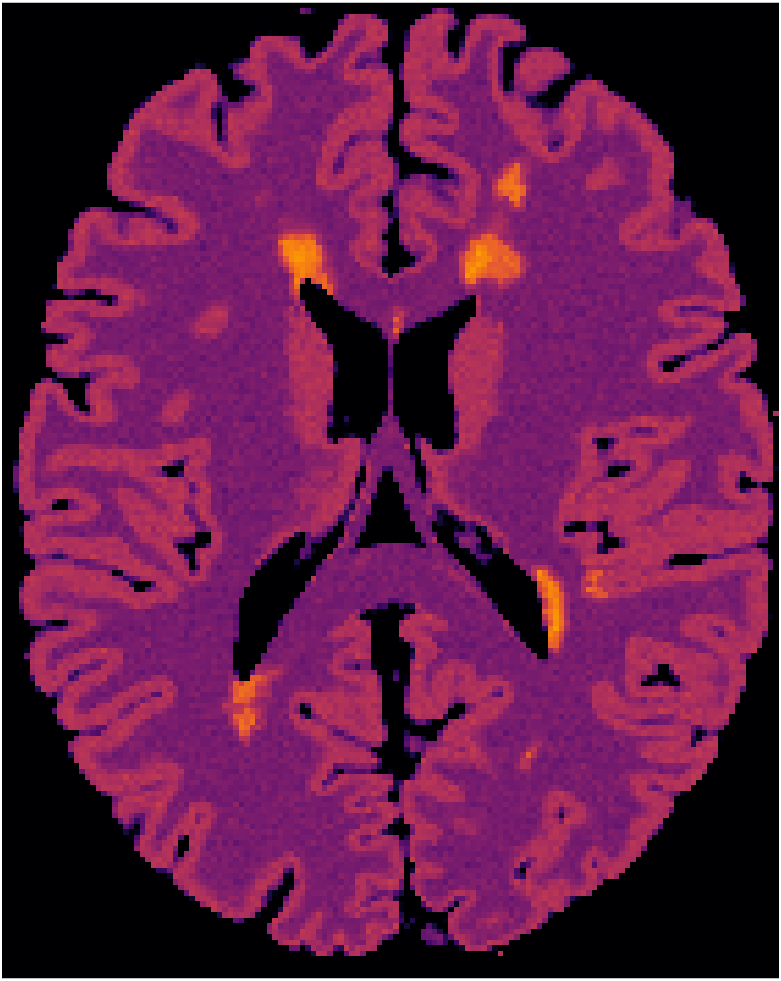
\includegraphics[height=\fullheight]{simflair-s=01.png}\caption{WMH 2017 (1)}\end{subfigure}
  \begin{subfigure}{0.25\textwidth}\centering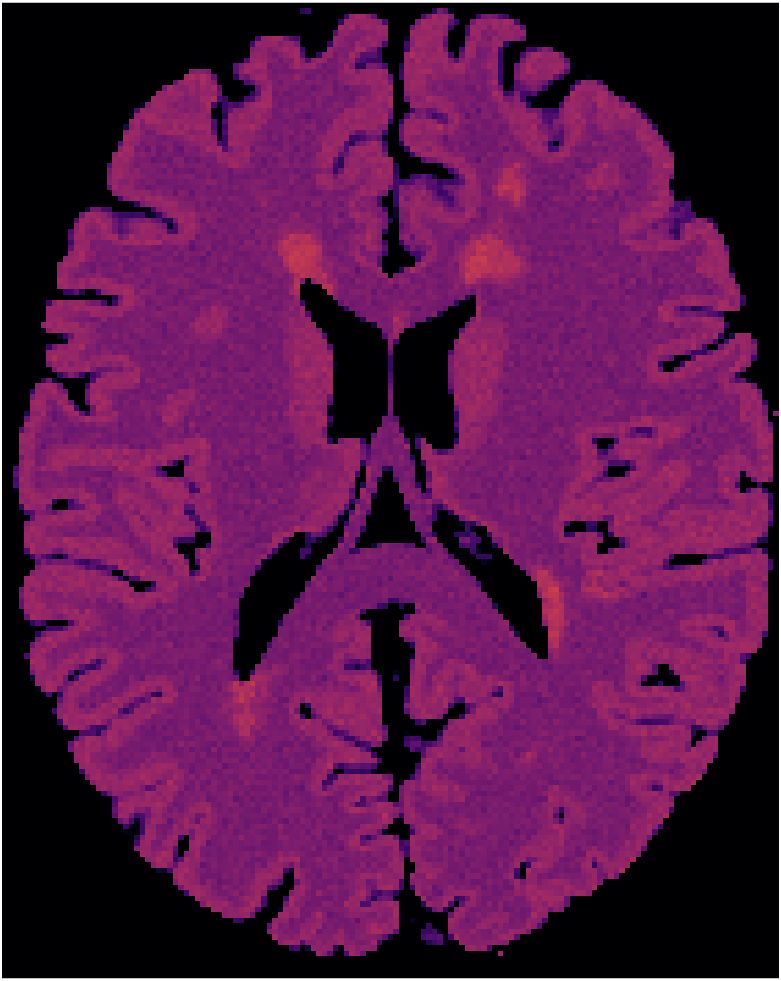
\includegraphics[height=\fullheight]{simflair-s=02.png}\caption{WMH 2017 (2)}\end{subfigure}
  \begin{subfigure}{0.25\textwidth}\centering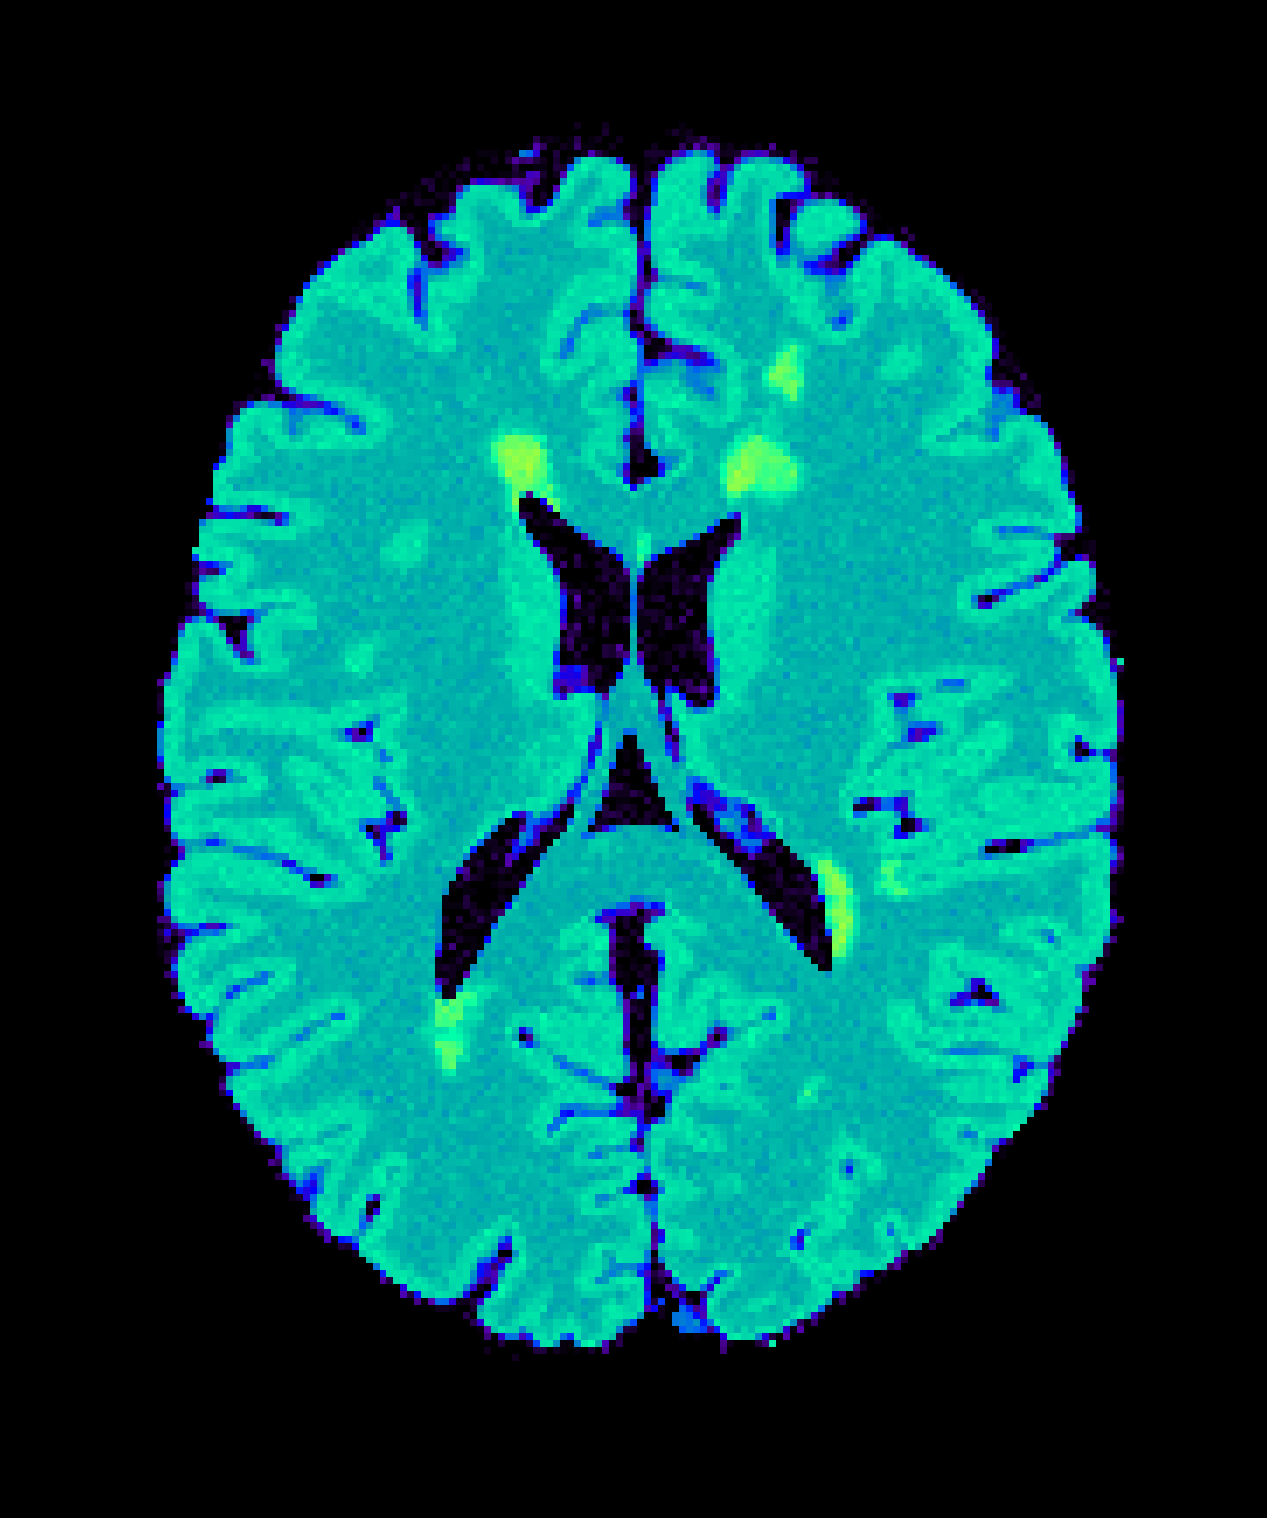
\includegraphics[height=\fullheight]{simflair-s=03.png}\caption{WMH 2017 (3)}\end{subfigure}\\[0.5em]
  \begin{subfigure}{0.25\textwidth}\centering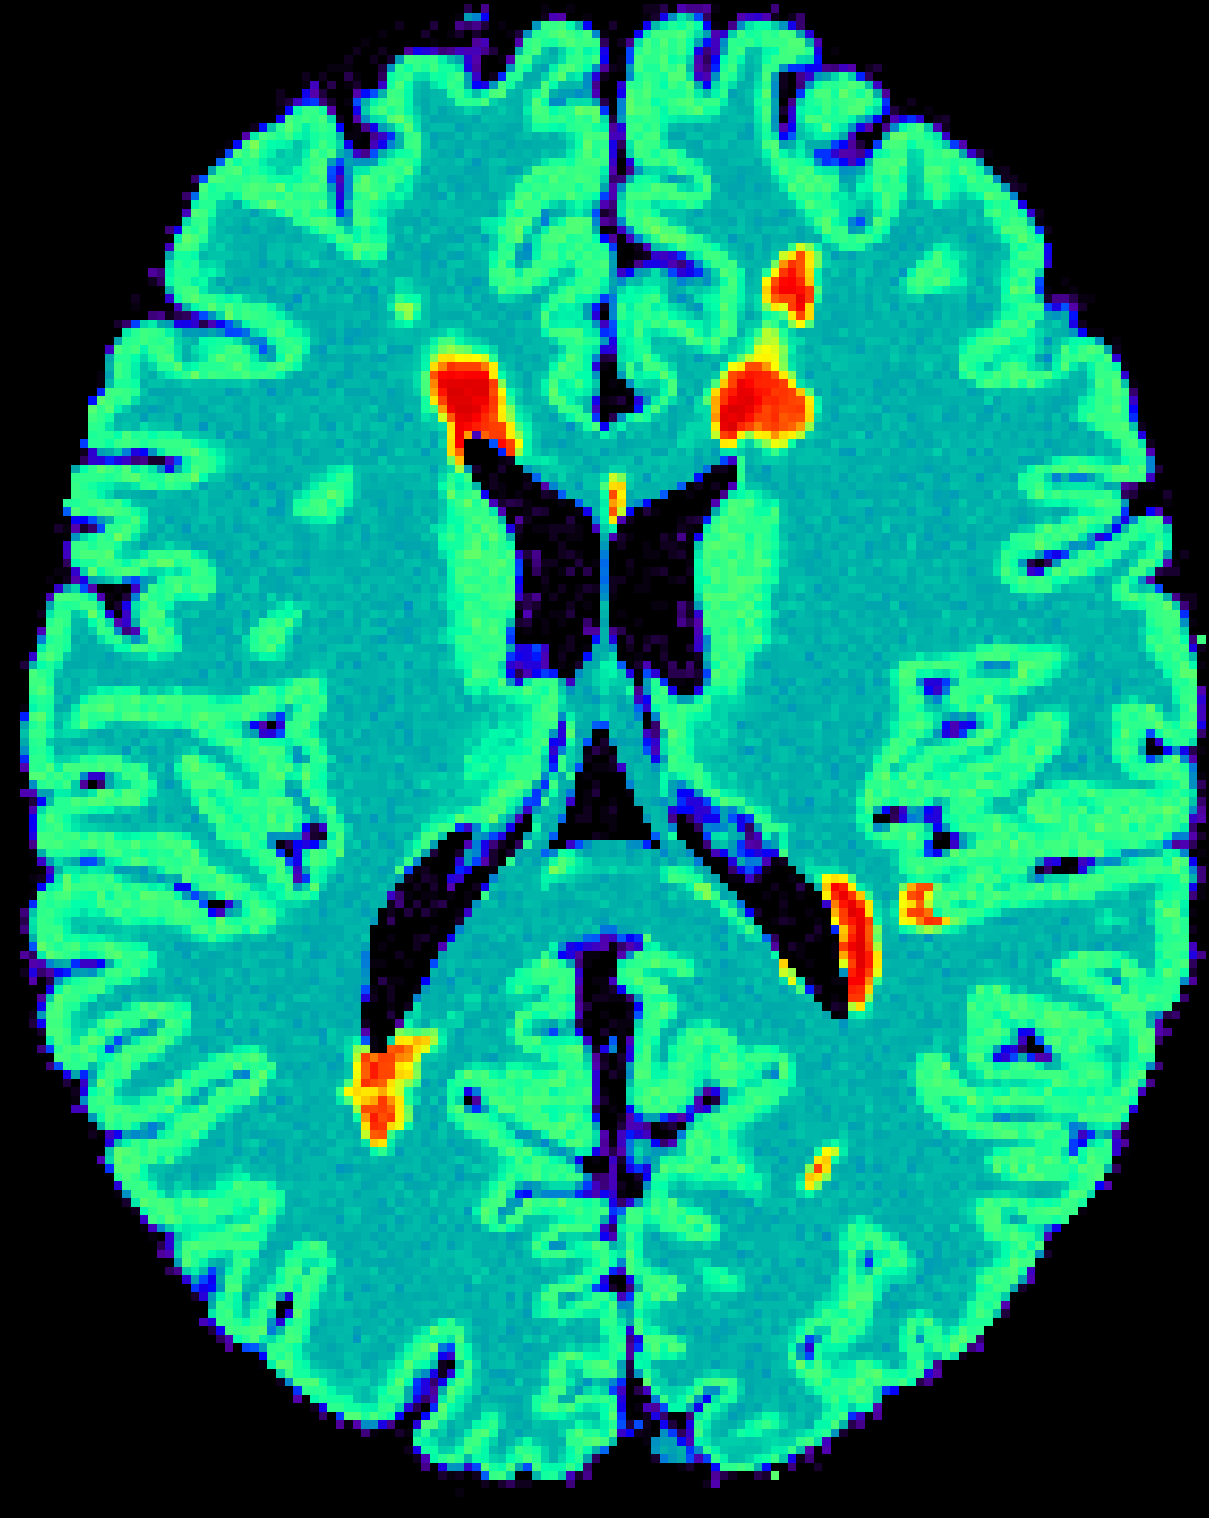
\includegraphics[height=\fullheight]{simflair-s=04.png}\caption{MS  2016 (1)}\end{subfigure}
  \begin{subfigure}{0.25\textwidth}\centering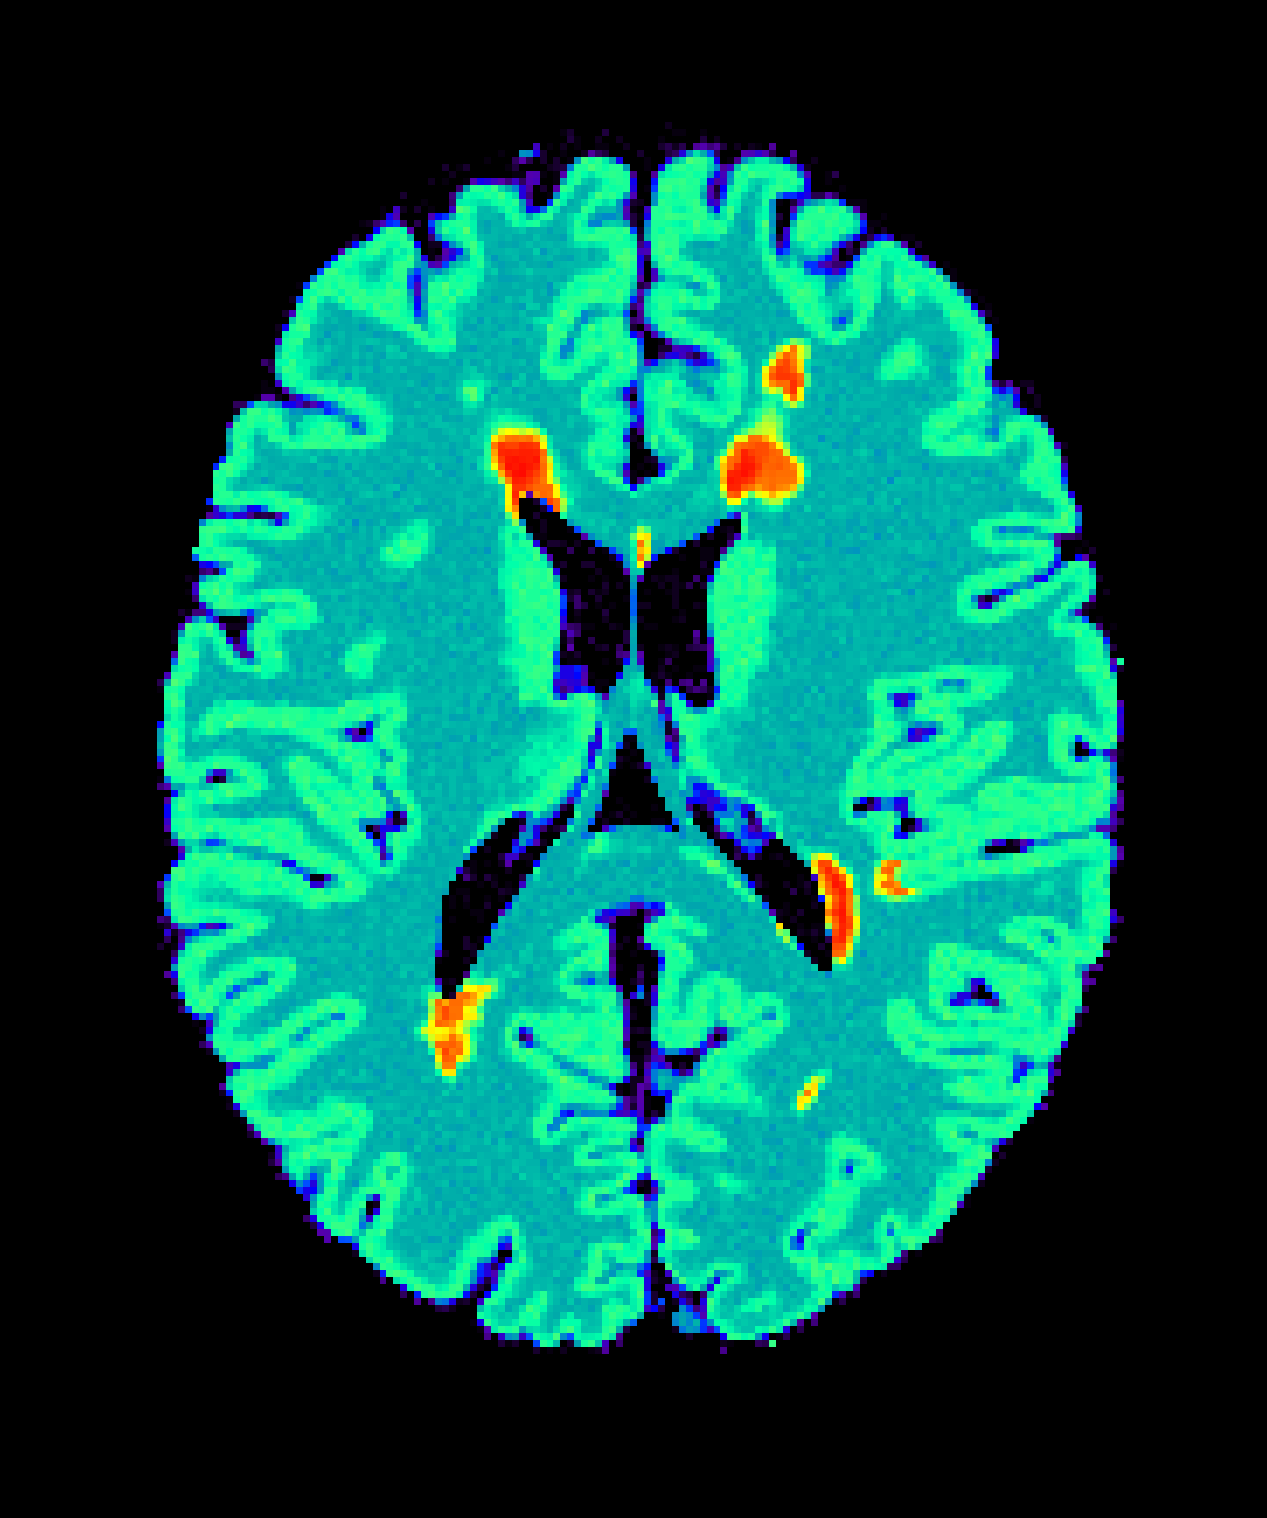
\includegraphics[height=\fullheight]{simflair-s=05.png}\caption{MS  2016 (2)}\end{subfigure}
  \begin{subfigure}{0.25\textwidth}\centering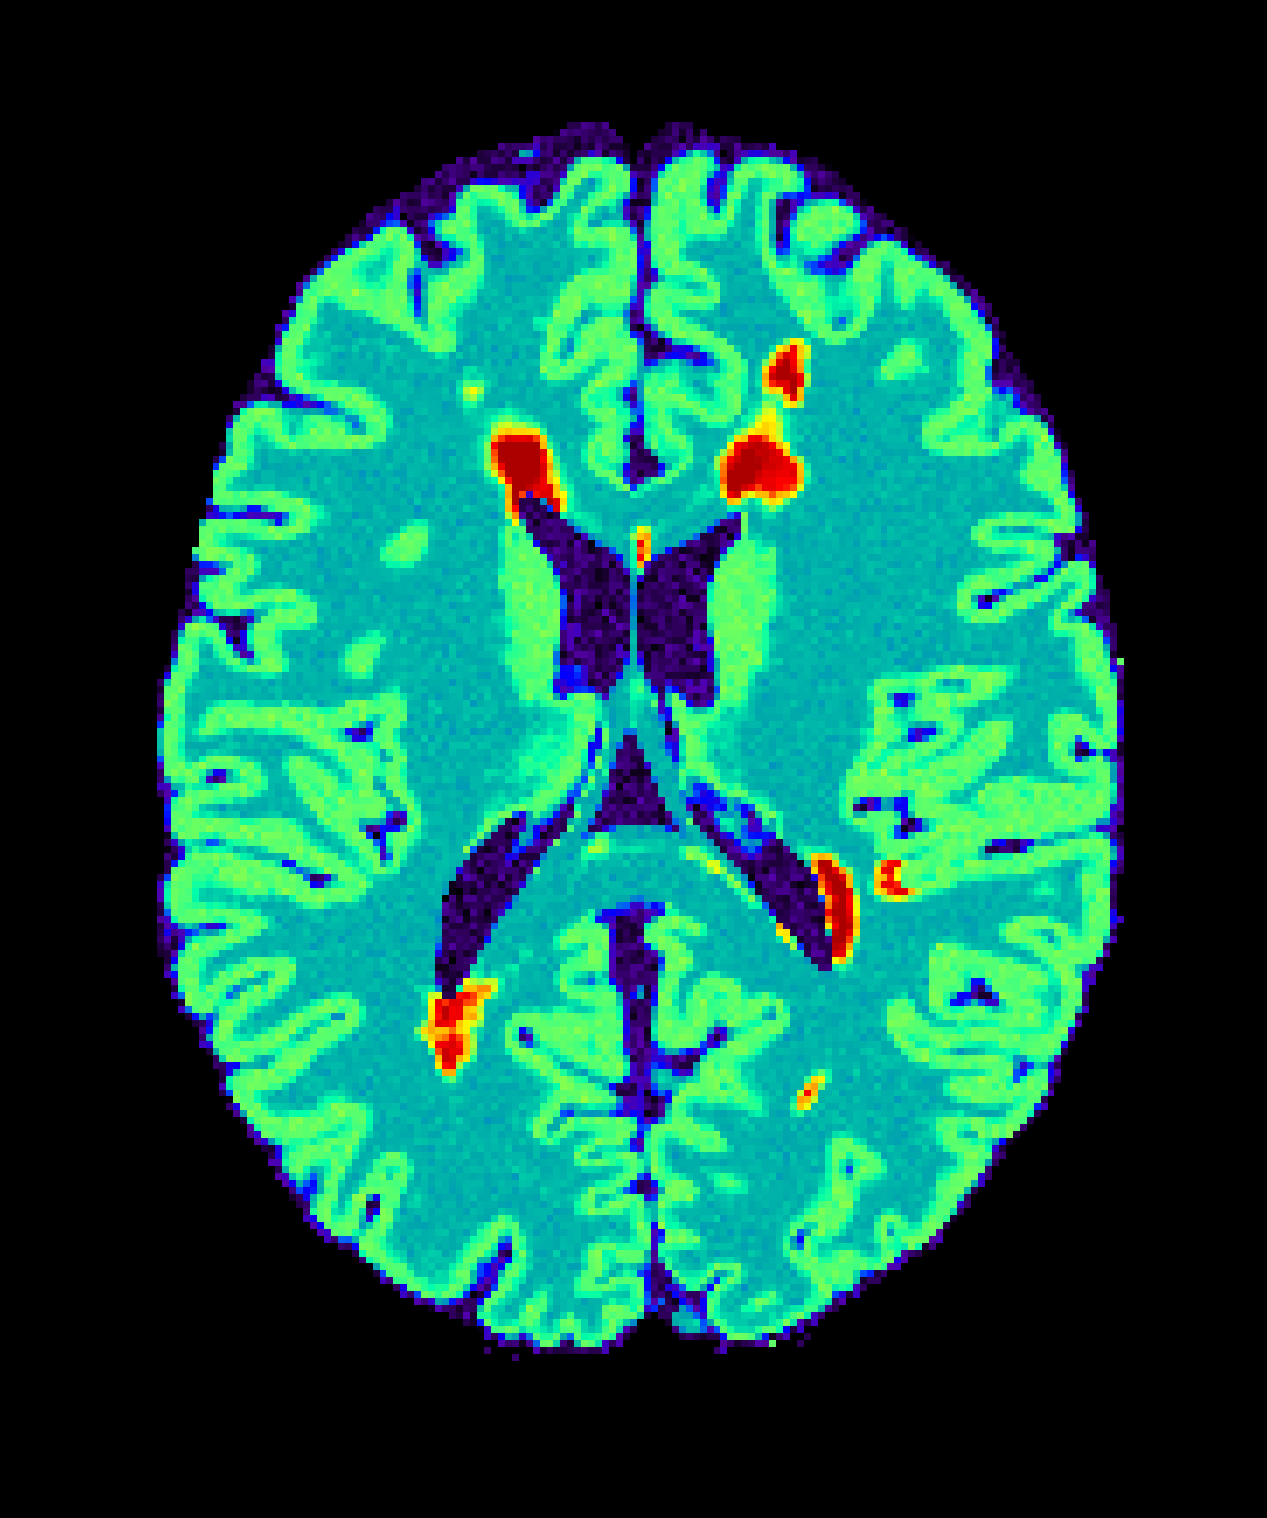
\includegraphics[height=\fullheight]{simflair-s=06.png}\caption{MS  2016 (3)}\end{subfigure}\\[0.5em]
  \begin{subfigure}{0.25\textwidth}\centering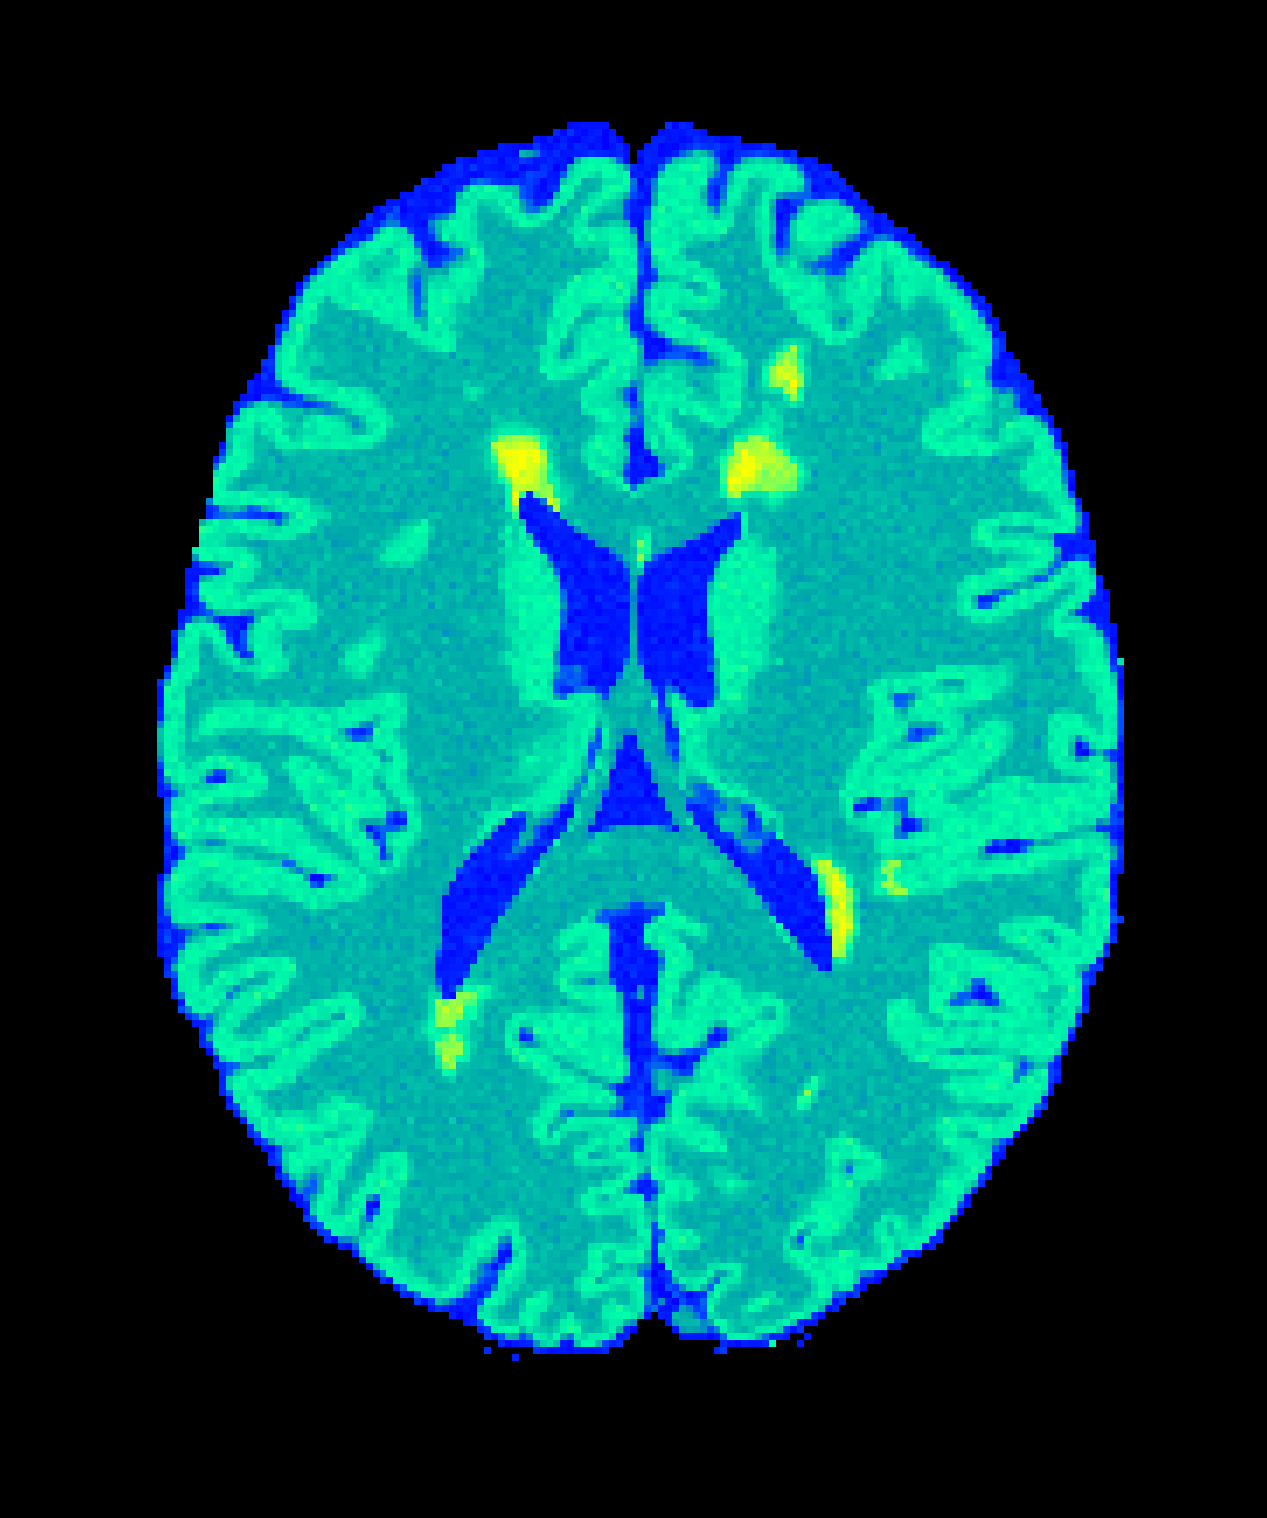
\includegraphics[height=\fullheight]{simflair-s=08.png}\caption{MS  2008 UNC}\end{subfigure}
  \begin{subfigure}{0.25\textwidth}\centering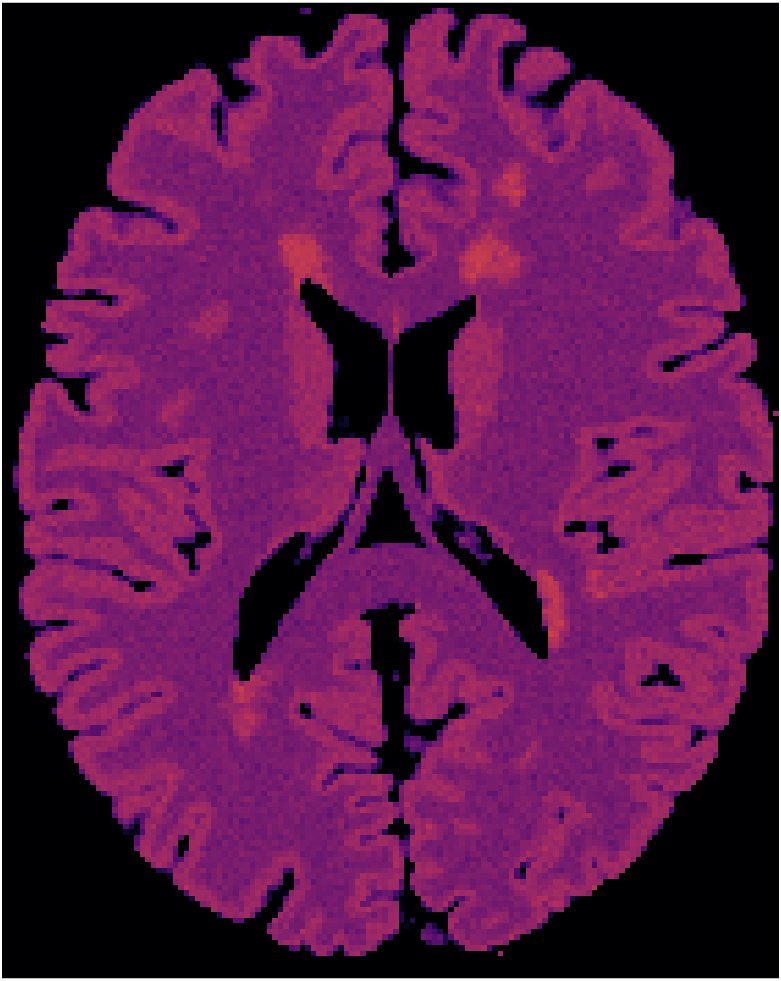
\includegraphics[height=\fullheight]{simflair-s=09.png}\caption{ISBI MS 2015}\end{subfigure}
  \begin{subfigure}{0.25\textwidth}\centering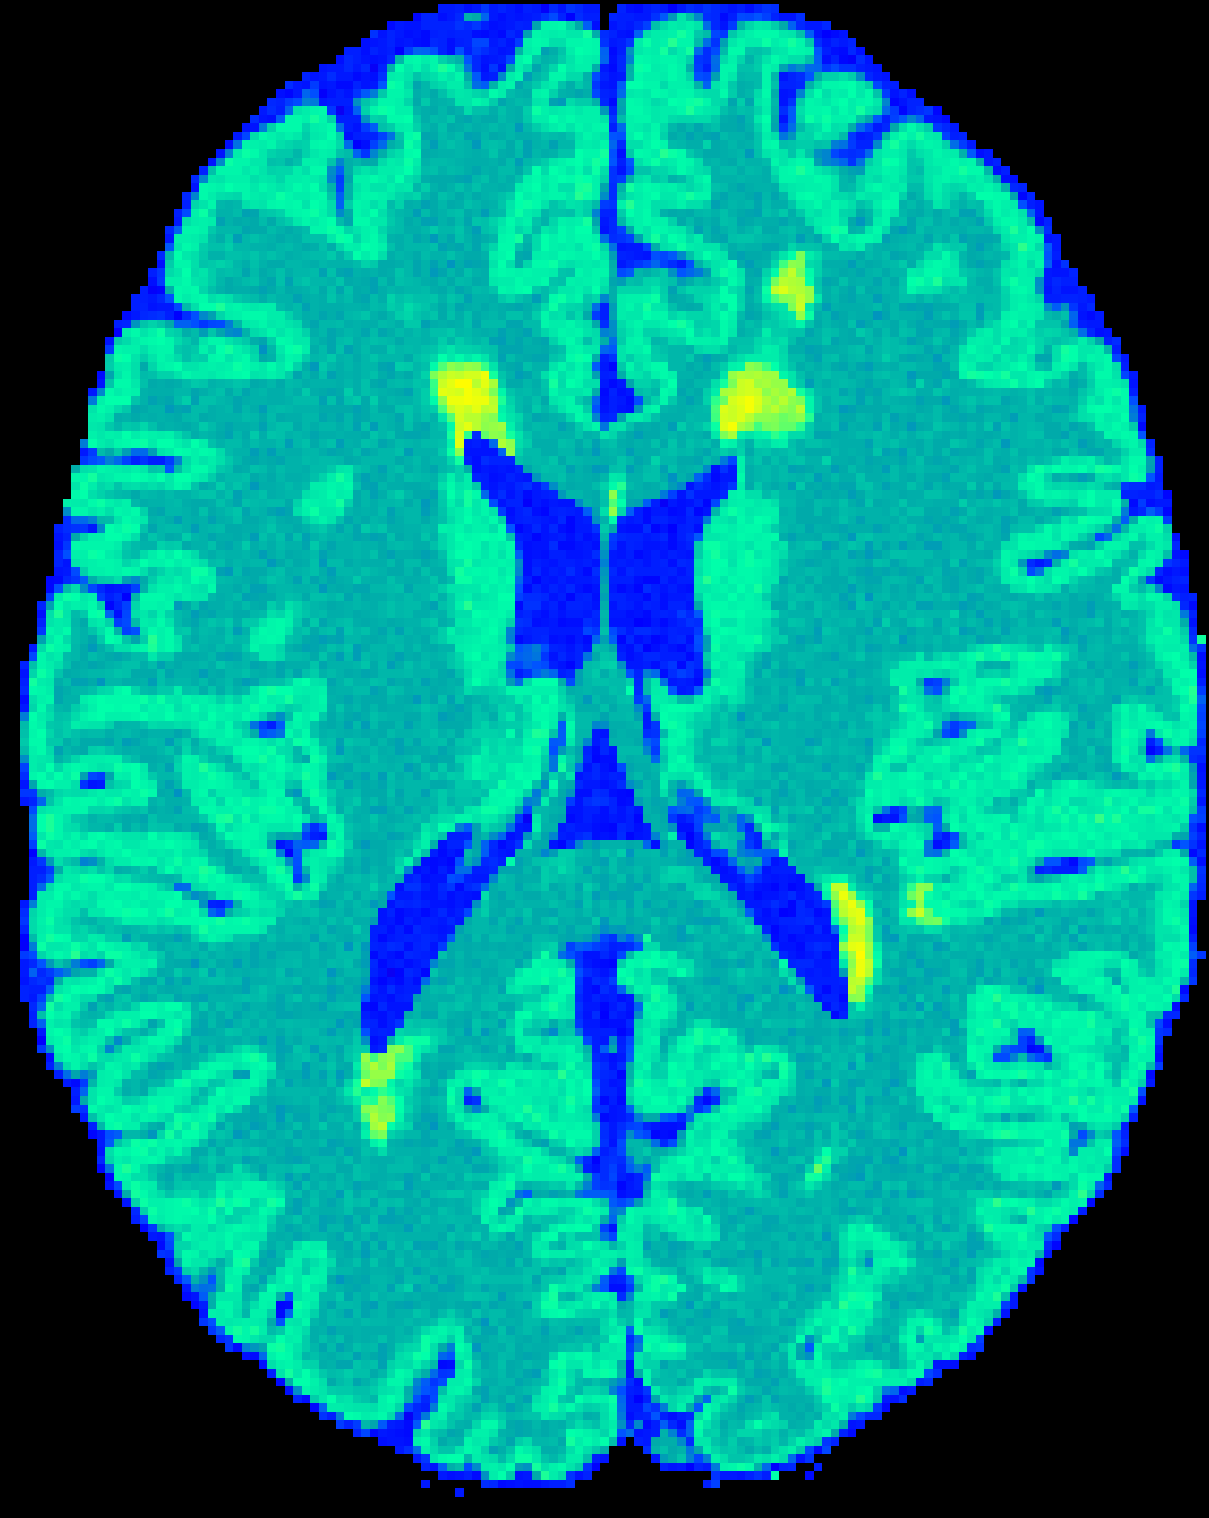
\includegraphics[height=\fullheight]{simflair-s=10.png}\caption{In-House    }\end{subfigure}\\[0.5em]
  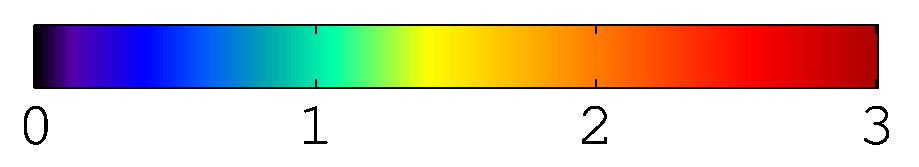
\includegraphics[width=0.25\textwidth]{hcbar-NIH3-0-3}
  \caption{Simulated FLAIR images using scan parameters from the experimental database. Colourmap is arbitrary but consistent.}
  \label{fig:simflair}
\end{figure}

%%%%%%%%%%%%%%%%%%%%%%%%%%%%%%%%%%%%%%%%%%%%%%%%%%%%%%%%%%%%%%%%%%%%%%%%%%%%%%%%%%%%%%%%%%%%%%%%%%%%
\section{Histogram Equalization Properties}




% --------------------------------------------------------------------------------------------------
% ==================================================================================================
%%%%%%%%%%%%%%%%%%%%%%%%%%%%%%%%%%%%%%%%%%%%%%%%%%%%%%%%%%%%%%%%%%%%%%%%%%%%%%%%%%%%%%%%%%%%%%%%%%%%
